%% This is summary of moose use cases.

\def\ghight{0.15\paperheight}
\def\gwidth{12cm}
\edef\figwidth{0.1\textwidth}

\begin{tikzpicture}
    \node[] (spineful_neuron) { 
        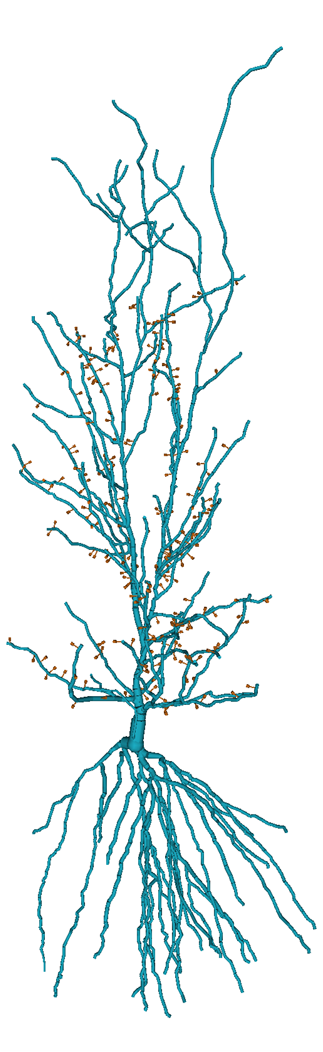
\includegraphics[height=\ghight]{./images/neuron_with_spine.png}
    };
\end{tikzpicture} \hfill %
\begin{tikzpicture}
    \node [] (moose_cell) {
        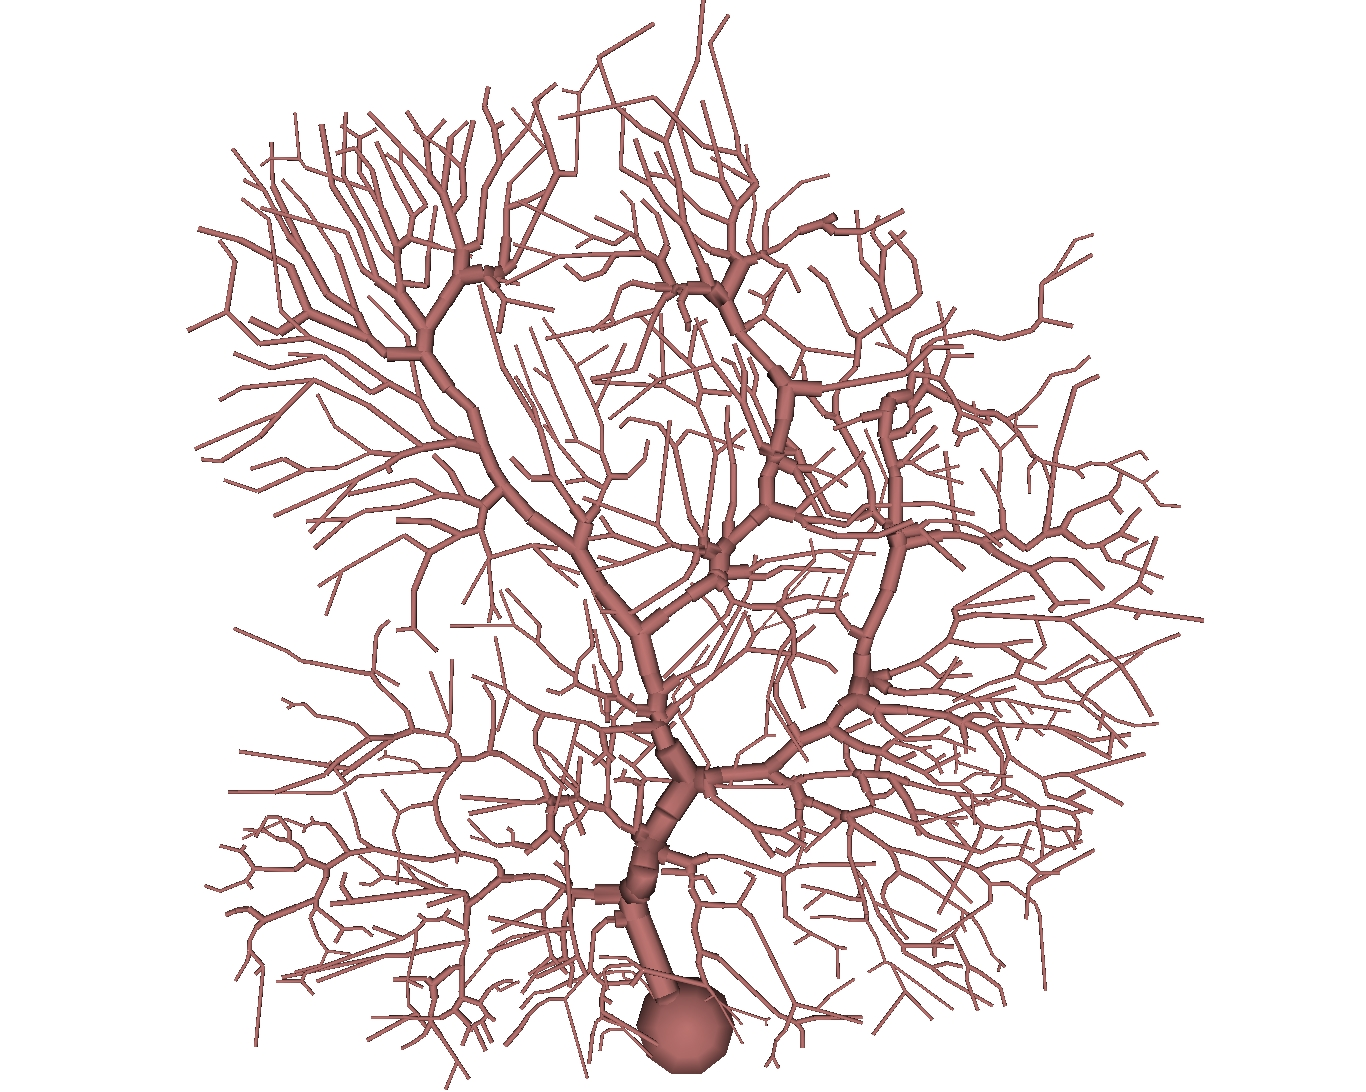
\includegraphics[height=\ghight]{./images/_1_7.jpeg}
    };
    %\node [text width=\figwidth,below=3.5cm] (captionA) {\CAPTION{Single Neuron Model}};
\end{tikzpicture} \hfill %
\begin{tikzpicture}
    % Now embed this neuron into a network.
    \node[] (subha1) {
        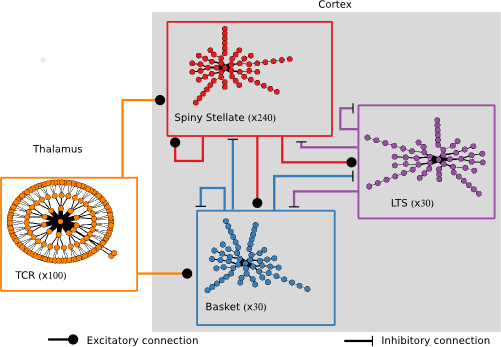
\includegraphics[height=\ghight]{./images/subha.png}
    };
\end{tikzpicture} \hfill %
\begin{tikzpicture}
    \node [] (subha) {
        \includegraphics[height=\ghight]{./images/reduced_model_pyramidical_cells.png}
    };
\end{tikzpicture} \hfill %
\begin{tikzpicture}
    \node[] (olfaction) {
        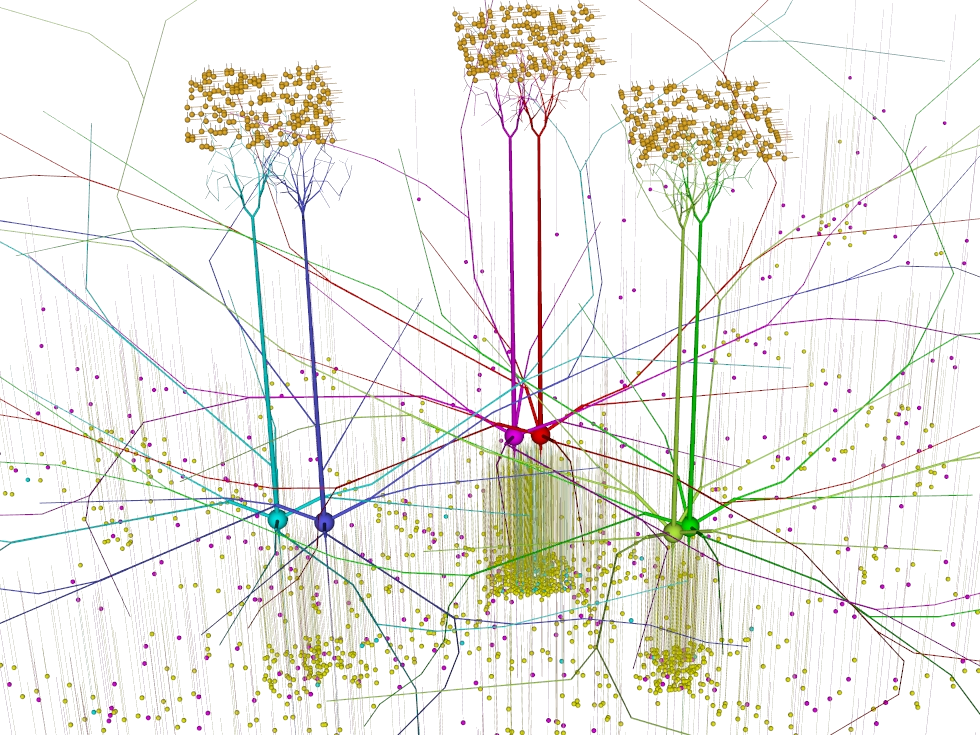
\includegraphics[height=\ghight]{./images/fullmodel_moogli.png}
    };
    %\node [text width=\figwidth, below=2.7cm] (captionB) {\CAPTION{Olfactory bulb model}};
\end{tikzpicture} \hfill %
\begin{tikzpicture}
    \node[] (projectb) {
        \includegraphics[height=\ghight]{./images/thalamocortical.png}
    };
\end{tikzpicture} \hfill %
\begin{tikzpicture}
    \node[] (chem_in_spine) { 
        \includegraphics[height=\ghight, width=20cm]{./images/psd_model.png}
    };
\end{tikzpicture} %

